% Define document class
\documentclass[twocolumn]{aastex631}
\usepackage{showyourwork}
\usepackage{multirow}
\usepackage{nicefrac}

% Glossaries
\usepackage[acronym,toc]{glossaries}
\newcommand*\myglsentry[1]{%
  \ifglsused{#1}{%
    \glsentryshort{#1}%
  }{%
    \glsentrylong{#1}%
  }%
}
\newacronym{scc}{SCC}{squamous cell carcinoma}
\newacronym{hnscc}{HNSCC}{head and neck \myglsentry{scc}}
\newacronym{opscc}{OPSCC}{oropharyngeal \myglsentry{scc}}
\newacronym{ctv}{CTV}{clinical target volume}
\newacronym{ctv-n}{CTV-N}{elective \myglsentry{ctv}}
\newacronym{lnl}{LNL}{lymph node level}
\newacronym{hpv}{HPV}{human papilloma virus}
\newacronym{hmm}{HMM}{hidden Markov model}
\newacronym{rv}{RV}{random variable}
\newacronym{dag}{DAG}{directed acyclic graph}
\newacronym{mcmc}{MCMC}{Markov chain Monte Carlo}
\newacronym{ti}{TI}{thermodynamic integration}
\newacronym{bic}{BIC}{Bayesian information criterion}
\newacronym{bn}{BN}{Bayesian network}
\newacronym{ct}{CT}{computed tomography}
\newacronym{mri}{MRI}{magnetic resonance imaging}
\newacronym{pet}{PET}{positron emission tomography}
\newacronym{fna}{FNA}{fine needle aspiration}
\newacronym{clb}{CLB}{Centre Leon Bérard}
\newacronym{usz}{USZ}{University Hospital Zurich}
\newacronym{isb}{ISB}{Inselspital Bern}

% Cross-referencing
\usepackage{hyperref}
\AtEndPreamble{\usepackage{cleveref}}

% Begin!
\begin{document}

% Title
\title{Modelling the Lymphatic Metastatic Progression Pathways of OPSCC from Multi-Institutional Datasets}

% Author list
\author{Roman Ludwig}
\author{Jean-Marc Hoffmann}
\author{Bertrand Pouymayou}
\author{Panagiotis Balermpas}
\author{Lauence Bauwens}
\author{Vincent Grégoire}
\author{Roland Giger}
\author{Jan Unkelbach}

% Abstract
\begin{abstract}
    The \gls{ctv-n}\glsunset{ctv} definition in \gls{hnscc}\glsunset{scc} is currently based mostly on the prevalence of lymphatic metastases in different \glspl{lnl} based on the primary tumor location. In this work, we present an extension to a probabilistic model for lymphatic metastatic spread developed earlier that can quantify the risk for microscopic nodal involvement based on individual diagnoses. The extension is based on the same formalism of \glspl{hmm} as the original model, but in addition to the \glspl{lnl} I, II, III, and IV, it also covers the \glspl{lnl} V and VII of the ipsilateral neck. Moreover, we infer which pathways of lymphatic spread to model from clinical lymphatic progression patterns of 681 patients from three institutions. The extended model may allow for a more personalized \gls{ctv-n} definition based on a patient's individual state of disease. The \gls{hmm} uses a collection of hidden binary \glspl{rv} -- one for each \gls{lnl} -- to model a patient's state of lymphatic involvement. Clinical diagnoses and/or pathological examinations of resected \glspl{lnl} represent the observed binary \glspl{rv} corresponding to the unobservable true state of nodal disease. A \gls{dag} with parametrized edges is used to compute the transition matrix of the \gls{hmm} and consequently the (log-)likelihood of the diagnoses of 681 patients, given a set of spread parameters. Based on the defined likelihood function, \gls{mcmc} sampling is then used to infer a distribution over the model's parameters. T-category is model by assuming that, on average, patients with late T-category tumors are diagnosed at a later time compared to patients with early T-category tumors. Using \gls{ti} and the \gls{bic} we compare models based on different \glspl{dag} and demonstrate the accuracy and precision of the best-performing model. When extended to the contralateral side, this model may form the basis of future guidelines of elective \gls{ctv} definition.
\end{abstract}

% Main body
\section{Introduction}
\label{sec:intro}

When treating \gls{hnscc}, either with radiotherapy or via surgery, the aim is to irradiate or resect as much of the present malignancies as possible. This includes the primary tumor mass and metastases that are sufficiently large to be detected using in-vivo imaging modalities such as \gls{ct}, \gls{mri}, or \gls{pet}. But it also includes regions of possible microscopic spread, which these modalities cannot detect, to increase the patient's probability of cure \cite{poortmans_internal_2020,murthy_prostate-only_2021}. Microscopic disease can currently only be observed by a pathological examination of the tissue. Consequently, clinicians that are presented with cancer patients need to routinely assess the risk of microscopic involvement in parts of the body that appear clinically node negative.

This work concerns itself with \gls{opscc}, which commonly spreads lymphatically. The only two publicly available datasets on nodal involvement patterns in \gls{opscc}, at the time of writing, show that 80\% of patients where either cN+ or -- if available -- pN+ \cite{ludwig_dataset_2022}. Since the exact number and location of lymph nodes varies from patient to patient, the nodes are grouped into anatomically defined \glspl{lnl}. These levels are then often irradiated or resected prophylactically due to the risk of harboring occult metastases despite negative findings from imaging modalities. In current clinical practice, \gls{ctv-n} definition is instead mostly based on guidelines \cite{gregoire_ct-based_2003,gregoire_delineation_2014,gregoire_delineation_2018,eisbruch_intensity-modulated_2002,biau_selection_2019,chao_determination_2002,vorwerk_guidelines_2011,ferlito_elective_2009} that are derived from the observed prevalence of involvement in an \gls{lnl} for a given tumor location.

These guidelines, however, do not account for the personal risk of the patients that may depend greatly on their diagnosis. E.g., macroscopic metastases detected via \gls{pet} in the \glspl{lnl} II and III may increase the risk for occult disease in \gls{lnl} IV over the case of a patient who presents with a clinically N0 neck.

A model for estimating the risk of microscopic disease, given a personal diagnosis based on \glspl{bn} was previously developed \cite{pouymayou_bayesian_2019} and subsequently adapted to make use of \glspl{hmm} to include T-category in an intuitive manner \cite{ludwig_hidden_2021}. These models were trained on a dataset of early T-category (T1 and T2) patients that could be reconstructed from \cite{sanguineti_defining_2009}. Since this publication only includes details about the involvement of the ipsilateral \glspl{lnl} I, II, III, and IV, the models were limited to these nodal levels as well.

With the publication of larger and more detailed datasets \cite{ludwig_dataset_2022}, the risk estimation models may be extended as well to include the additionally reported \glspl{lnl} V and VII. This work aims to do that and at the same time demonstrate the capability 
of the previously introduced \gls{hmm} to adapt to real patient data from a multi-centric cohort of XXX \gls{opscc} patients.

\section{Previous Work}
\label{sec:previous_work}

\subsection{Lymphatic Spread as Hidden Markov Model}
\label{subsec:previous_work:spread_as_hmm}

We have introduced a probabilistic model for lymphatic metastatic tumor progression based on \glspl{bn} in \cite{pouymayou_bayesian_2019} and based off of this an improved model using \glspl{hmm} in \cite{ludwig_hidden_2021}. We will briefly recap the \acrlong{hmm} below.

A patient's state of (hidden) lymphatic involvement at time $t$ is described as a collection of binary \glspl{rv}, one for each of the $V$ \glspl{lnl}:
%
\begin{equation}
    \mathbf{X}[t] = \left( X_v[t] \right) \qquad v \in \left\{ 1,2, \ldots, V \right\}
\end{equation}
%
Where each of the \glspl{lnl} can be in the state $X_v=0$ (\texttt{FALSE}), meaning \gls{lnl} $v$ is healthy, or in the state $X_v=1$ (\texttt{TRUE}), indicating the \gls{lnl} harbors metastases.

The transition from one time-step to another is governed by the transition probability $P\left( \mathbf{X}[t+1]=\boldsymbol{\xi}_i \mid \mathbf{X}[t]=\boldsymbol{\xi}_j \right)$, which can conveniently be collected into a transition matrix when we enumerate all $2^V$ distinct possible states $\boldsymbol{\xi}_i$ with $i \in \left\{ 1,2, \ldots, 2^V \right\}$ of lymphatic involvement:
%
\begin{equation}
    \mathbf{A} = \left( A_{ij} \right) = \left( P\left( \mathbf{X}[t+1]=\boldsymbol{\xi}_i \mid \mathbf{X}[t]=\boldsymbol{\xi}_j \right) \right)
\end{equation}
%
The term $P\left( \boldsymbol{\xi}_i \mid \boldsymbol{\xi}_j \right)$ describes the probability to transition from the hidden state of lymphatic involvement $\boldsymbol{\xi}_j$ to the state $\boldsymbol{\xi}_i$ within between the time $t$ and $t+1$. Using a \gls{dag} as depicted in \cref{fig:graph_with_obs}, we can parameterize this transition probability in the following way:
%
\begin{equation}
    \label{eq:transition_prob}
    P\left( \boldsymbol{\xi}_i \mid \boldsymbol{\xi}_j \right) = \prod_{v \leq V} Q\left( \xi_{iv} ; \xi_{jv} \right) P \left( \xi_{iv} \mid \left\{ \xi_{jr} \right\}_{r \in \operatorname{pa}(v)} \right)^{1 - \xi_{jv}}
\end{equation}
%
In this equation, we have denoted \glspl{lnl} that are parents of \gls{lnl} $v$ with the symbol $r\in\operatorname{pa}(v)$. Also, $\xi_{iv}$ denotes the value that \gls{lnl} $v$ takes on when the patient is in state $\boldsymbol{\xi}_i$. Lastly, the term $Q(a;b) \in \{ 0,1 \}$ is there only to 

\begin{figure}
    \centering
    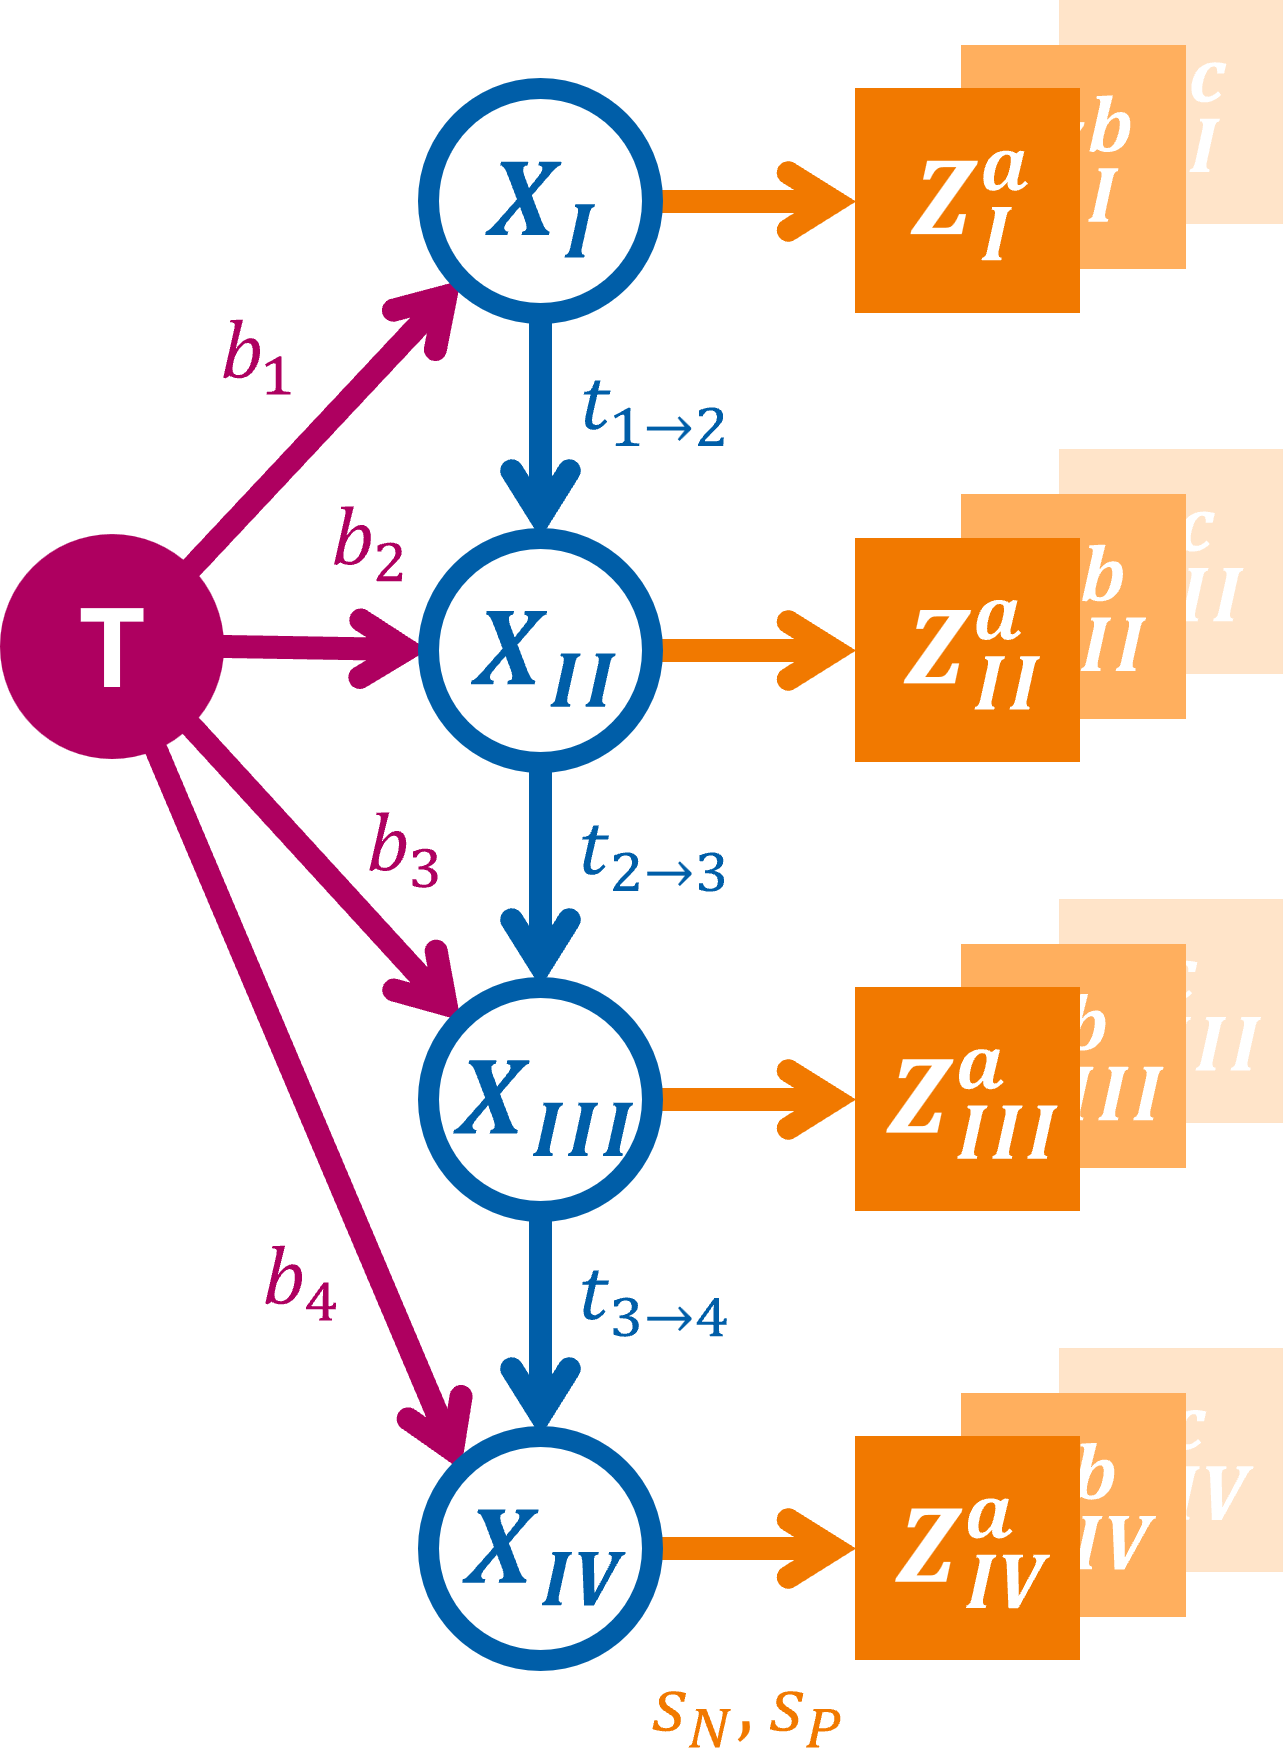
\includegraphics[width=0.6\linewidth]{figures/graph_with_obs.png}
    \caption{\Gls{dag} representing a possible abstraction of the lymphatic network comprising the tumor (red shaded circle) and \glspl{lnl} I through IV as hidden binary \glspl{rv} (blue outlined circles). Attached to each of these is the corresponding observed \gls{rv} (orange shaded squares). Lymphatic flow is depicted in the form of parameterized arrows (red and blue) that represent the probability of spread along the respective arc per time-step. Sensitivity and specificity (orange arrows) connect the hidden \glspl{rv} to the diagnosis.}
    \label{fig:graph_with_obs}
\end{figure}

Diagnosis and true state of a patient are formally connected via the sensitivity $s_N$ and specificity $s_P$ of the used diagnostic modality. In clinical practice, these modalities are \gls{ct}, \gls{mri}, or \gls{pet} scan, but it may also include information from biopsies after a \gls{fna} or other techniques to detect lymphatic metastases. For each \gls{lnl} $v$ the conditional probability table of $P\left( Z_v \mid X_v \right)$ looks like this:

\noindent
\begin{center}
    \begin{tabular}{|cc|cc|}
        \hline
        & & \multicolumn{2}{c|}{$X$} \\
        & & 0 & 1 \\
        \hline
        \multirow{2}{*}{$Z$} & 0 & $s_p$ & $1 - s_N$ \\
        & 1 & $1 - s_P$ & $s_N$ \\
        \hline
    \end{tabular}
\end{center}

Consequently, the conditional probability to observe a diagnosis $\mathbf{Z}=\boldsymbol{\zeta}_\ell$, given a hidden involvement state $\mathbf{X}=\boldsymbol{\xi}_k$ is a matrix $\mathbf{B}$ made up of products of terms from the table above:
%
\begin{equation} \label{eq:transition_matrix}
    \mathbf{B} = \left( B_{k\ell} \right) = \prod_{v=1}^V P\left( Z_v = \zeta_{\ell v} \mid X_v[t_\text{D}] = \xi_{kv} \right)
\end{equation}

If multiple diagnostic modalities $\mathcal{O} \in \{ \text{MRI}, \text{CT}, \ldots \}$ are used, one can compute an observation matrix $\mathbf{B}^\mathcal{O}$ for each of these modalities and combine them via an outer product into a joint observations matrix:
%
\begin{equation}
    \mathbf{B} = \mathbf{B}^\text{MRI} \otimes \mathbf{B}^\text{CT} \otimes \ldots
\end{equation}

We define the time $t=0$ to be the moment just before a patient's tumor formed, and hence $X_v[t=0]=0 \,\,\, \forall v$. However, using this definition, we cannot know how many time-steps have passed until $t_\text{D}$, when the patient was diagnosed with cancer. We can only make the assumption that a patients with an earlier T-category tumor was \emph{probably} diagnosed after fewer time-steps than a patient with a late T-category tumor. We can use this information by marginalizing over the diagnose times $t_\text{D}$ of patients in different T-categories using different prior distributions over the diagnose time. E.g., $P \left( t=t_D \mid \text{early} \right)$ for early T-category patients (T1 \& T2) and $P \left( t=t_D \mid \text{late} \right)$ for late T-category patients (T3 \& T4). Throughout this work we will use binomial distributions for these probability mass functions, mainly because they have a plausible shape for this purpose and only a single parameter.
%
\begin{equation}
    P \left( t = t_D \mid \text{T-cat.} \right) = \operatorname{B}(t_\text{max},p_\text{T-cat.})
\end{equation}
%
Here, the parameter $p_\text{early}$ can be interpreted as the probability that the patient will be diagnosed at time-step $t+1$ given they are in time-step $t$. We will use as a latest time-step $t_\text{max} = 10$.

\subsection{The Likelihood Function}
\label{subsec:previous_work:likelihood}

Using the definitions up to this point, we can compute a vector of likelihoods for every possible diagnosis:
%
\begin{equation} \label{eq:likelihood_vec}
\begin{split}
    \boldsymbol{\ell} &= \big( P\left( \mathbf{Z} = \boldsymbol{\zeta}_i \right) \big) \\
    &= \sum_{t=0}^{t_{max}} \left[ \boldsymbol{\pi} \cdot \mathbf{A}^t \cdot \mathbf{B} \right] \cdot P \left( t \mid \text{T-cat.} \right)
\end{split}
\end{equation}
%
This likelihood implicitly depends on how we parameterize the arcs of the \gls{dag} underlying the model and the parameterization of the distribution over diagnosis times. If we use the graph displayed in \cref{fig:graph_with_obs}, we can write down a conditional probability table for \gls{lnl} $X_3$ being healthy or metastatic, based on the state of the parent \gls{lnl} $\operatorname{pa}(3) = 2$:

\noindent
\begin{center}
    \begin{tabular}{|cc|cc|}
        \hline
        & & \multicolumn{2}{c|}{$X_2$} \\
        & & 0 & 1 \\
        \hline
        \multirow{2}{*}{$X_3$} & 0 & $1 - b_3$ & $(1 - b_3)(1 - t_{23})$ \\
        & 1 & $b_3$ & $1 - b_3 - t_{23} + b_3 t_{23}$ \\
        \hline
    \end{tabular}
\end{center}

Similar tables can be written for all other \glspl{lnl}. The terms in these conditional probability tables can then be used to compute the transition probability between to particular states $\boldsymbol{\xi}_i$ and $\boldsymbol{\xi}_j$ as in \cref{eq:transition_prob}. Computing this quantity for all possible transitions subsequently yields the transition matrix $\mathbf{A}$ as described in \cref{eq:transition_matrix}.

Together with the parametrizations of the distributions over the diagnosis time, the parameters that make up the transition matrix $\mathbf{A}$ comprises the set of model parameters:
%
\begin{equation}
    \boldsymbol{\theta} = \left( \left\{ b_v \right\}, \left\{ t_{vr} \right\}, p_\text{early}, p_\text{late} \right) \quad \text{with} \quad \genfrac{}{}{0pt}{2}{v\leq V}{r\in\operatorname{pa}(v)}
\end{equation}

To infer these parameters from a dataset of $N$ \gls{hnscc} patients $\boldsymbol{\mathcal{D}} = \left( d_1, d_2, \ldots, d_N \right)$, we compute the data log-likelihood:
%
\begin{equation} \label{eq:log_likelihood}
    \log\mathcal{L} \left( \boldsymbol{\mathcal{D}} \mid \boldsymbol{\theta} \right) = \sum_{i=1}^N \log P \left( \mathbf{Z} = d_i \right)
\end{equation}
%
Which effectively amounts to computing the element-wise logarithm of the likelihood vector $\boldsymbol{\ell}$ from \cref{eq:likelihood_vec} and summing up the entries that correspond to each of the patients $d_i$ for $i\leq N$. 

Using this log-likelihood function one may now employ a variety of inference methods to learn the parameters of the model that best describe the observed data. After that, the main task of of personalizing the \gls{ctv-n} definition is to predict the probability of the hidden possible states $\boldsymbol{\xi}_k$ given the diagnosis $d^\star=\boldsymbol{\zeta}_\ell$ of a new patient. Using Bayes' theorem, we get
%
\begin{equation}
    P\left( \mathbf{X}=\boldsymbol{\xi}_k \mid \mathbf{Z}=\boldsymbol{\zeta}_\ell \right) = \frac{P\left( \boldsymbol{\zeta}_\ell \mid \boldsymbol{\xi}_k \right) P\left( \boldsymbol{\xi}_k \mid \boldsymbol{\theta} \right)}{\sum_{r=1}^{2^V} P\left( \boldsymbol{\zeta}_\ell \mid \boldsymbol{\xi}_r \right) P\left( \boldsymbol{\xi}_r \mid \boldsymbol{\theta} \right) }
\end{equation}
%
The described model along with the inferred parameters $\boldsymbol{\hat{\theta}}$ will yield an estimate (or multiple estimates) for the ``prior'' in the above equation $P\big( \boldsymbol{\xi}_k \mid \boldsymbol{\hat{\theta}} \big)$.

\section{Methods}
\label{sec:methods}

\subsection{Parameter Inference}
\label{subsec:methods:inference}

We use \gls{mcmc} sampling to draw parameter samples $\boldsymbol{\hat{\theta}}_i$ for $i \leq S$ from the likelihood described in \cref{eq:log_likelihood} (i.e. the unnormalized posterior distribution over the parameters $\boldsymbol{\theta}$, since we used a uniform prior in this work).

More specifically, we use the Python implementation \texttt{emcee} \cite{foreman-mackey_emcee_2013} and two sample proposal mechanisms based on differential evolution moves \cite{ter_braak_differential_2008,nelson_run_2013} for sampling. Instead of proposing and then accepting or rejecting individual parameter samples one after the other (as in the classical Metropolis-Hastings algorithm), the \texttt{emcee} implementation makes use of an ensemble of $W$ so-called ``walkers''. This gives rise to $W$ parallel chains of samples that mutually influence each others proposal such that the sampling proceedure overall is \emph{affine invariant}. This means that scaling the parameter space along any dimension has no effect on the performance of the \gls{mcmc}.

For the experiments in this work, we used $W = 20 \cdot k$ walkers, where $k$ is the dimensionaliry of the parameter space $\boldsymbol{\Theta}$. After an initial ``burn-in'' phase, during which all drawn samples are discarded because they are not yet independent from the initial state, we continued sampling for another 200 steps of which we discarded every 10th to be left with $S = 20 \cdot W$ samples.

These $S$ parameter estimates are then used to compute expectation values of estimates that depend on the parameters $\boldsymbol{\theta}$ through an integral over the parameter space $\boldsymbol{\Theta}$:
%
\begin{equation}
    \begin{aligned}
        \mathbb{E}_p \left[ f \right] &= \int_{\boldsymbol{\Theta}} p(\boldsymbol{\theta}) f(\boldsymbol{\theta}) d\boldsymbol{\theta} \\
        &\approx \frac{1}{S} \sum_{i=1}^S f \big( \boldsymbol{\hat{\theta}}_i \big)
    \end{aligned}
\end{equation}
%
Alternatively, the individual $\hat{f}_i = f\big( \boldsymbol{\hat{\theta}}_i \big)$ can be used to plot histograms over the distribution of $f$. We will do so in \cref{sec:results} to show distributions over prevalence predictions and risk computations.

Another relevant model parameter that needs to be set for the inference process, is the maximum number of time-steps we used for the evolution of the system. We set this value to $t_\text{max} = 10$, such that $t \in \{ 0, 1, 2, \ldots, 10 \}$. The binomial ``success probability'' used to fix the shape of the early T-category's time-prior was set to $p_\text{early} = 0.3$.

\subsection{Model Comparison}
\label{subsec:methods:comparison}

\begin{table*}
    \centering
    \begin{tabular}{ | c | c | c | }
        \hline
        $K_\text{1v2}$ & $\ln{K_\text{1v2}}$ & support for $\mathcal{M}_1$ \\
        \hline
        $< 10^0$ & $< 0$ & negative evidence (supports $\mathcal{M}_2$) \\
        $10^0$ to $10^{\nicefrac{1}{2}}$ & 0 to 1.15 & barely worth a mention \\
        $10^{\nicefrac{1}{2}}$ to $10^1$ & 1.15 to 2.3 & substantial \\
        $10^1$ to $10^{\nicefrac{3}{2}}$ & 2.3 to 3.45 & strong \\
        $10^{\nicefrac{3}{2}}$ to $10^2$ & 3.45 to 4.6 & very strong \\
        $> 10^2$ & $> 4.6$ & decisive \\
        \hline
    \end{tabular}
    \caption{Interpretation of Bayes factors and their natural logarithms in terms of their support for or against one of the two compared models as introduced by Harold Jeffreys \cite{jeffreys_theory_1998}.}
    \label{table:bayes_factor}
\end{table*}

The aim of this work is to refine the graph structure underlying our risk model introduced in the previous section. This \gls{dag} determines the number of parameters of the model as well as how exactly the transition matrix $\mathbf{A}$ is parameterized. To compare different models that are based on different \glspl{dag}, e.g. models $\mathcal{M}_1$ and $\mathcal{M}_2$, in a Bayesian setting, we need to compute the probabilities of these models, given the data $\boldsymbol{\mathcal{D}}$:
%
\begin{equation}
    P \left( \mathcal{M}_i \mid \boldsymbol{\mathcal{D}} \right) = \frac{P \left( \boldsymbol{\mathcal{D}} \mid \mathcal{M}_i \right) P \left( \mathcal{M}_i \right)}{ P \left( \boldsymbol{\mathcal{D}} \right) }
\end{equation}
%
If we assume all models $\mathcal{M}_i$ for $i \in \{ 1,2 \}$ to have the same \emph{a priori} probability -- meaning in this case $P (\mathcal{M}_1) = P (\mathcal{M}_2)$ -- then we can compute the so-called \emph{Bayes factor} of the two models as the ratio of their likelihoods. The interpretation of the values for different Bayes factors is given in \cref{table:bayes_factor}. It is defined as follows:
%
\begin{equation}
    K_\text{1v2} = \frac{P \left( \mathcal{M}_1 \mid \boldsymbol{\mathcal{D}} \right)}{P \left( \mathcal{M}_2 \mid \boldsymbol{\mathcal{D}} \right)} = \frac{P \left( \boldsymbol{\mathcal{D}} \mid \mathcal{M}_1 \right)}{P \left( \boldsymbol{\mathcal{D}} \mid \mathcal{M}_2 \right)}
\end{equation}
%
These likelihoods are commonly called the \emph{model evidence} or \emph{marginal likelihood}. The latter because computing it involves marginalizing the data likelihood over all model parameters:
%
\begin{equation} \label{eq:evidence}
    E_\mathcal{M} = P \left( \boldsymbol{\mathcal{D}} \mid \mathcal{M} \right) = \int_{\boldsymbol{\Theta}} P\left( \boldsymbol{\mathcal{D}} \mid \boldsymbol{\theta}, \mathcal{M} \right) p(\boldsymbol{\theta} \mid \mathcal{M}) d\boldsymbol{\theta}
\end{equation}
%
However, this quantity is often very hard to compute or even intractable, due to the high dimensionality of the parameter space $\boldsymbol{\Theta}$. In our case, the number of dimensions ranges from $k=9$ for the \emph{base graph} to $k=11$ for the \emph{winning graph}. A brute-force integration over a unit cube with this many dimensions is inefficient and error prone, which is why we resorted to \gls{ti} for computing the (log-)evidence.

Below, we will briefly outline the main concept behind this algorithm. An intuitive and extensive derivation of \gls{ti} is given by \cite{aponte_introduction_2022}.

We start by taking the logarithm of the model evidence $E$ and subtract a zero from it in the form of the term $0 = \ln \int p(\boldsymbol{\theta} \mid \mathcal{M}) d\boldsymbol{\theta}$. Further, we can multiply the distribution over the parameters $\boldsymbol{\theta}$ inside this integral by $1 = P \left( \boldsymbol{\mathcal{D}} \mid \boldsymbol{\theta}, \mathcal{M} \right)^{\beta=0}$. Subsequently, we can write the logarithm of the evidence as an integral over a derivative:
%
\begin{equation} \label{eq:ti}
    \begin{aligned}
        \ln E &= \ln \int P \left( \boldsymbol{\mathcal{D}} \mid \boldsymbol{\theta}, \mathcal{M} \right)^{\beta=1} p \left( \boldsymbol{\theta} \mid \mathcal{M} \right) d\boldsymbol{\theta} - \ln E_0 \\
        &= \int_0^1 \frac{d}{d\beta} \ln E_\beta d\beta
    \end{aligned}
\end{equation}
%
Where we have used the (unnormalized) \emph{power posterior} $p_\beta \left( \boldsymbol{\theta} \mid \boldsymbol{\mathcal{D}}, \mathcal{M} \right) = P \left( \boldsymbol{\mathcal{D}} \mid \boldsymbol{\theta}, \mathcal{M} \right)^\beta p \left( \boldsymbol{\theta} \mid \mathcal{M} \right)$ to compute the respective evidence $E_\beta = \int p_\beta \left( \boldsymbol{\theta} \mid \boldsymbol{\mathcal{D}}, \mathcal{M} \right) d\boldsymbol{\theta}$.

The derivatives of the log-evidences $\ln E_\beta$ are essentially expectation values of the data log-likelihood under the power posteriors of the corresponding value for $\beta$. They can be computed using \gls{mcmc}:
%
\begin{equation}
    \begin{aligned}
        \frac{d}{d\beta} \ln E_\beta &= \int p_\beta \left( \boldsymbol{\theta} \mid \boldsymbol{\mathcal{D}}, \mathcal{M} \right) \ln P \left( \boldsymbol{\mathcal{D}} \mid \boldsymbol{\theta}, \mathcal{M} \right) d\boldsymbol{\theta} \\
        &= \mathbb{E} \left[ \ln P \left( \boldsymbol{\mathcal{D}} \mid \boldsymbol{\theta}, \mathcal{M} \right) \right]_{ p_\beta \left( \boldsymbol{\theta} \mid \boldsymbol{\mathcal{D}}, \mathcal{M} \right) } \\
        &\approx \frac{1}{S} \sum_{i=1}^S \ln P \left( \boldsymbol{D} \mid \hat{\boldsymbol{\theta}}_{\beta i}, \mathcal{M} \right) =: \mathcal{A}_\text{MC} \left( \beta \right)
    \end{aligned}
\end{equation}
%
The integral in \cref{eq:ti} can then be computed via a trapezoidal rule using the $\mathcal{A}_\text{MC}$ to yield a  numerical approximation of the model evidence:
%
\begin{equation}
    \ln E \approx \frac{1}{2} \sum_{j=0}^{R-1} \left( \beta_{j+1} - \beta_j \right) \cdot \big( \mathcal{A}_\text{MC} (\beta_{j+1}) + \mathcal{A}_\text{MC} (\beta_j) \big)
\end{equation}
%
This estimate gets better for more samples $S$ per sampling from the power posterior $p_\beta$ but more importantly it gets better for a tighter spacing of the values for $\beta$ within the interval $[0,1]$. The variable $\beta$ is also often referred to as an \emph{inverse temperature}, due to its origins in statistical physics. Often when performing \gls{ti}, the most drastic changes in the values of the $\mathcal{A}_\text{MC}$ occur at high temperatures (meaning $\beta$ very close to zero), while the changes become smaller and smaller for lower temparatures ($\beta$ towards one). It is therefore efficient to space the \emph{temperature ladder} unevenly, e.g. according to a fifth order power rule:
%
\begin{equation} \label{eq:power_rule}
    \beta_j = \left( j / R \right)^5 \qquad j \in \{ 0, 1, 2, \ldots, R \}
\end{equation}
%
For the \glspl{ti} that were performed in this work we used such a fifth order power rule with 64 steps, meaning that $R=63$.

The process of computing the log-evidence using \gls{ti} was as follows: We randomly initialized the starting positions of the $W$ samplers in the ensemble within the $k$ dimensional unit cube $\boldsymbol{\Theta}$. Subsequently, for each $j \in \{ 0, 1, 2, \ldots, R=63 \}$ we drew samples from the corresponding power posterior with the value of $\beta_j$ set according to the power rule in \cref{eq:power_rule}. This sampling at point $j$ consisted of 1000 burn-in steps, followed by 200 steps, of which only every tenth was kept. The last position of the $W$ chains for the $j$-th $\beta$ value in the ladder was used to initialize the subsequent sampling round with $\beta_{j+1}$. Hence, after the computations are finished, we are left with $S = 20 \cdot W$ samples $\boldsymbol{\hat{\theta}}_{i,j}$ and respective log-likelihood $\hat{\ell}_{i,j}$ from each of the 64 power posteriors corresponding to the respective $\beta_j$. Subsequently, we numerically integrated the following quantity $S$ times:
%
\begin{equation}
    \ln \hat{E}_i = \frac{1}{2} \sum_{j=0}^{R-1} \left( \beta_{j+1} - \beta_j \right) \cdot \left( \hat{\ell}_{i,j} + \hat{\ell}_{i,j+1} \right)
\end{equation}
%
And then computed the mean and standard deviation of all the integrated $\ln \hat{E}_i$. We then used this for the log-evidence and its error.

Without derivation or insight, we would like to mention that the model evidence naturally balances a model's accuracy against its complexity. The value of $\ln E$ will generally be larger (i.e., less negative) if a model fits the data better than another while being similarily complex. On the other hand, if e.g. additional parameters are introduced without sufficiently improving how well the model explains the data, the evidence will penalize the increase in complexity.

An approximation to the evidence that also attempts to balance accuracy and complexity against each other is the heuristic called \gls{bic}. The negative one half of the \gls{bic} approximates the $\ln E$ via Lagrange's method \cite{bhat_derivation_2010} and yields an easy to compute estimate that may also be used to compare models, as long as its underlying assumptions are valid:
%
\begin{equation} \label{eq:bic}
    - \text{BIC} / 2 = \ln{\hat{\mathcal{L}}} - \frac{k}{2} \ln{N} \approx \ln{E}
\end{equation}
%
Here, $\hat{\mathcal{L}} = \max_{\boldsymbol{\theta}}{\left( \ln P \left( \boldsymbol{\mathcal{D}} \mid \boldsymbol{\theta} \right)\right)}$ is the maximum log-likelihood. The approximation is good, when the posterior distribution over the parameters $p\left( \boldsymbol{\theta} \mid \boldsymbol{\mathcal{D}} \right)$ is single-modal and falls quickly to zero from the maximum. Also, the number of datapoints $N$ needs to be much larger than the number of parameters $k$. We will see that for the models we consider here, the \gls{bic} is generally a good approximation and the conclusions drawn from comparing models using this metric can be reproduced reliably using the true model evidence computed with \gls{ti}.

\subsection{Reproducibility}
\label{subsec:methods:reproducibility}

The entire methodology used in this work is publicly available in the GitHub repository \href{https://github.com/rmnldwg/lynference}{\texttt{rmnldwg/lynference}}. Tagged references to specific versions of an inference pipeline allow reproducing the inferred parameters of the models described here. Every parameter necessary to reproduce such a pipeline is specified there in designated configuration files. It also defines the sequences of computations that constitute the pipeline that are mostly calls to commands of the \href{https://pypi.org/project/lyscripts/}{\texttt{lyscripts}} we published.

All figures in this work, like the risk predictions and prevalences we show histograms of, can be reproduced following the instructions of the GitHub repository underlying this publication \href{\GitHubURL}{\texttt{rmnldwg/graph-extension}}. It is based off of the \showyourwork project.

\section{Multicentric Dataset}
\label{sec:data}

The dataset $\boldsymbol{\mathcal{D}}$ that we used for inference is comprised of the detailed reports on lymphatic involvement patterns in \gls{opscc} patients treated at three different institutions in France and Switzerland: The \gls{clb} in Lyon (France), the \gls{isb}, and the \gls{usz} (both in Switzerland). We have previously published the patterns of nodal involvement for the \gls{usz} cohort \cite{ludwig_dataset_2022} and described its characteristics in detail \cite{ludwig_detailed_2022}. A large part of the \gls{clb} data underlies a publication on \gls{hpv} status in \gls{opscc} \cite{bauwens_prevalence_2021} that was kindly provided to us by Vincent Grégoire. The patient information on lymphatic metastatic involvement from the \gls{isb} cohort was sent to us by Roland Giger through a collaboration.

In total, the dataset contains 681 patients newly diagnosed with \gls{opscc} that were treated with either definitive radiotherapy or neck dissection. Pathologically assessed post-operative \gls{lnl} involvement was available for 393 of patients, while for the remainder the nodal involvement was assessed based on available diagnostic modalities. If multiple modalities were used to diagnose a patient's lymphatic involvement and conflicting conclusions were drawn from this, the conflicts were resolved by inferring the most likely state (healthy or metastatic) for each \gls{lnl} separately. To do so, we used literature values for the sensitivity and specificity of the diagnostic modalities \cite{de_bondt_detection_2007,kyzas_18f-fluorodeoxyglucose_2008}, which we also tabulated below.

\noindent
\begin{center}
    \begin{tabular}{|l|rr|}
        \hline
        \textbf{Modality} & \textbf{Specificity} & \textbf{Sensitivity} \\
        \hline
        \acrshort{ct} & 76\% & 81\% \\
        \acrshort{pet} & 86\% & 79\% \\
        \gls{mri} & 63\% & 81\% \\
        \acrshort{fna} & 98\% & 80\% \\
        Pathology & $\approx$ 100\% & $\approx$ 100\% \\
        \hline
    \end{tabular}
\end{center}

\section{Results}
\label{sec:results}

\begin{table*}
    \centering
    \variable{output/results_table.tex}
    \caption{Model comparison results from the base graph and the extended graph we chose as the ``winnning'' model. For both \glspl{dag} we show the log-evidence, computed via thermodynamic integration, the negative one half of the \gls{bic}, as well as the maximum log-likelihood that was encountered during the final \gls{mcmc} sampling round.}
    \label{table:evidence}
\end{table*}

\begin{figure*}
    \script{bg_core_prevs.py}
    \begin{centering}
        \includegraphics[width=\textwidth]{figures/bg_core_prevs.png}
        \caption{Prevalence of involvement as predicted by the base graph model for different scenarios involving the most commonly metastatic \glspl{lnl} II, III and IV (shaded histograms). The model's predictions are compared to Beta posteriors over the prevalence based on the frequency of the same scenarios and a uniform prior (slid lines). The top panel shows some selected scenarios with early T-category tumors and the bottom panel with late T-category.}
        \label{fig:bg_prevalences}
    \end{centering}
\end{figure*}

\subsection{Base Graph}
\label{subsec:results:base_graph}

For the base graph, we have plotted the predicted prevalence of involvement patterns in the investigated patient cohort for scenarios involving the most commonly metastatic \glspl{lnl} II, III and IV in \cref{fig:bg_prevalences}. This figure shows that this minimal graph is already capable of describing the most important parts of the observed data very well. The subsequent changes to the graph connections we investigated therefore focus on the improvements w.r.t. involvement patterns that include the \glspl{lnl} I, V, and VII that more rarely harbor occult disease.

\begin{figure}
    \script{comp_IandII_low_prevs.py}
    \begin{centering}
        \includegraphics[width=\linewidth]{figures/comp_IandII_low_prevs.png}
        \caption{Prevalence predictions of the winning extended graph (colored histograms) compared to the base graph (hatched histograms) for scenarios of nodal involvement in the levels I and II. The solid lines depict the Beta posterior over the prevalence based on a uniform prior and the number of patients matching the respective scenario in the data. The top and bottom panel show the same scenarios, but for early and late T-category respectively.}
        \label{fig:IandII_low_prevs}
    \end{centering}
\end{figure}

\begin{figure}
    \script{comp_IandII_high_prevs.py}
    \begin{centering}
        \includegraphics[width=\linewidth]{figures/comp_IandII_high_prevs.png}
        \caption{Histograms and Beta posteriors over the prevalence of involvement for \gls{lnl} II (with and without \gls{lnl} I being metastatic as well). The colored histograms depict the predictions of the extended graph, while the hatched ones show the same prediction for the base graph. The top panel displays the predictions and observations for early T-category patients, the bottom panel for late T-category ones.}
        \label{fig:IandII_high_prevs}
    \end{centering}
\end{figure}

\begin{figure}
    \script{comp_IIandVII_prevs.py}
    \begin{centering}
        \includegraphics[width=\linewidth]{figures/comp_IIandVII_prevs.png}
        \caption{Placeholder.}
        \label{fig:IIandVII_prevs}
    \end{centering}
\end{figure}

\begin{figure}
    \script{comp_IIIandV_prevs.py}
    \begin{centering}
        \includegraphics[width=\linewidth]{figures/comp_IIIandV_prevs.png}
        \caption{Placeholder.}
        \label{fig:IIIandV_prevs}
    \end{centering}
\end{figure}

\begin{figure}
    \script{comp_IVandV_prevs.py}
    \begin{centering}
        \includegraphics[width=\linewidth]{figures/comp_IVandV_prevs.png}
        \caption{Placeholder.}
        \label{fig:IVandV_prevs}
    \end{centering}
\end{figure}

\bibliography{bib}

\end{document}
